\subsection{Ablation: PCA dimension versus the full embedding}\label{sec:pca}
To test whether the inconclusive result depends on how strongly the embedding is compressed, we varied the
number of PCA components appended to the handcrafted features ($k\in\{2,4,8,16,32,64,128\}$) and also used the
full standardised 5{,}120-dimensional embedding without PCA, for both the raw-series and smoothed-series
embeddings. All other settings (frozen LightGBM hyperparameters, five seeds, folds) were unchanged, and
$k=0$ is the LightGBM baseline (Figure~\ref{fig:pca}, Table~\ref{tab:pca}).
\begin{figure}[H]\centering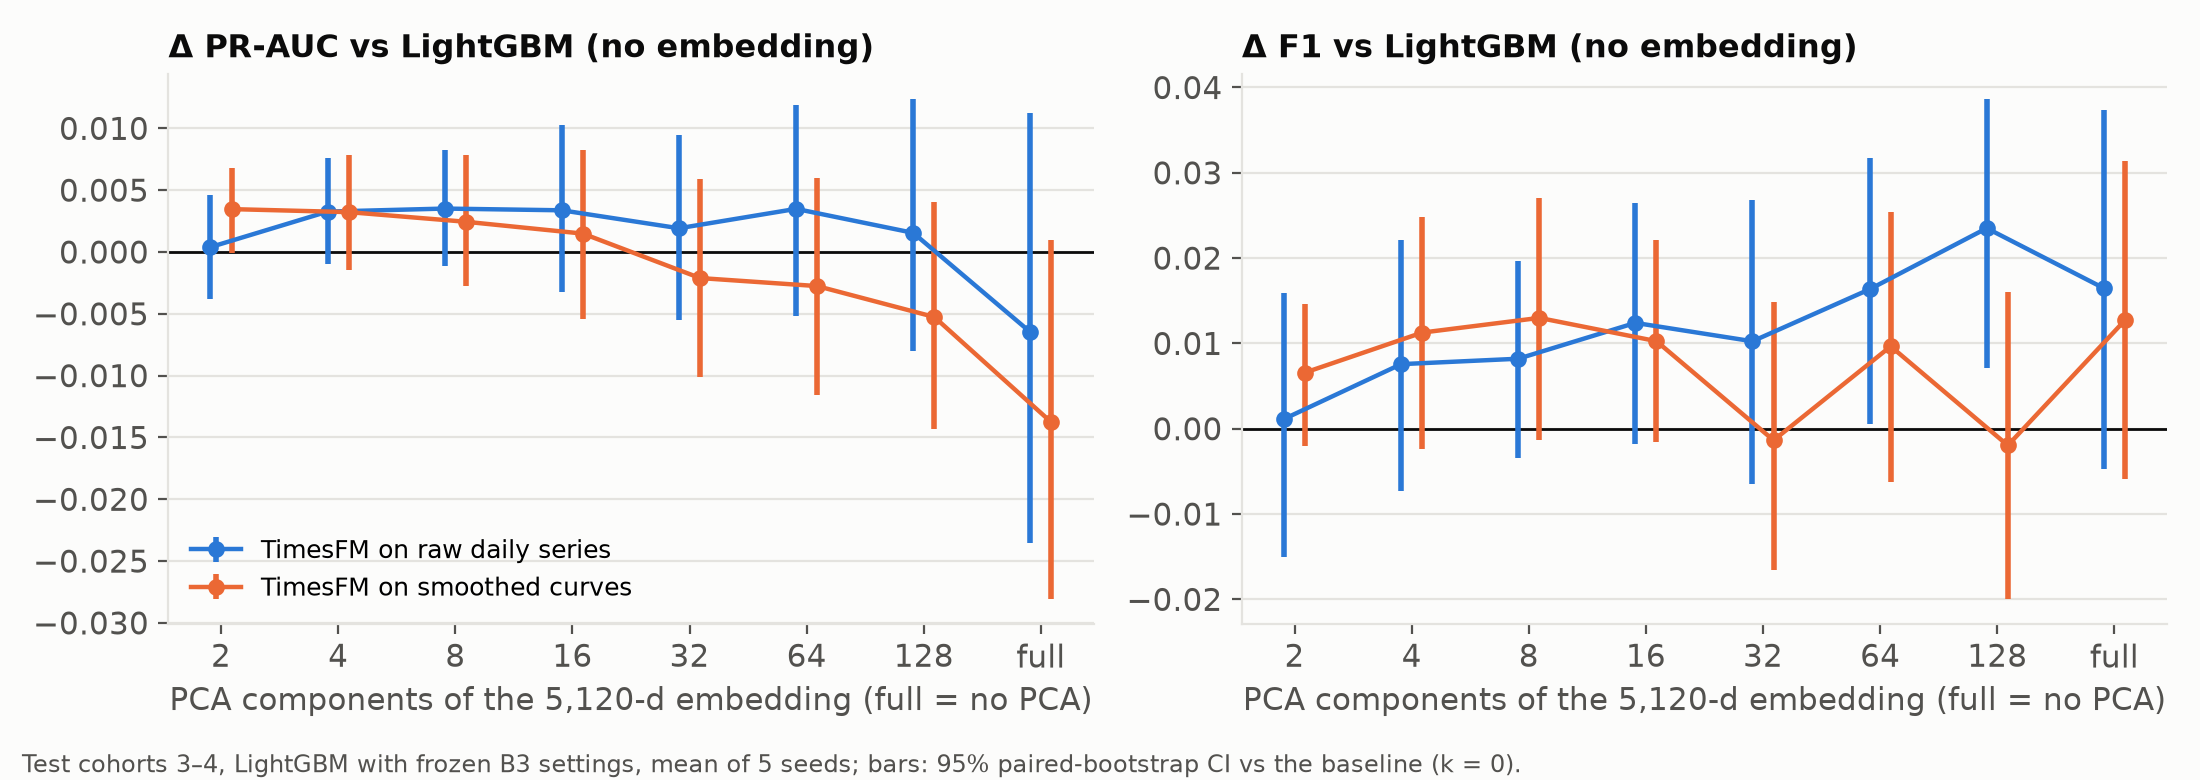
\includegraphics[width=\linewidth]{fig_pca_ablation.png}
\caption{Effect of the number of PCA components of the TimesFM-3 embedding on test PR-AUC and F1,
relative to the LightGBM baseline without embeddings. Bars are 95\% paired-bootstrap confidence intervals.}
\label{fig:pca}\end{figure}
\begin{table}[H]\centering\small\setlength{\tabcolsep}{4pt}
\begin{tabular}{llccccc}\toprule
Embedding & $k$ & Expl.\ var. & Val.\ PR-AUC & Test PR-AUC & $\Delta$PR-AUC [95\% CI] & $\Delta$F1 [95\% CI]\\\midrule
none (LightGBM) & 0 & -- & 0.537 & 0.472 & -- & --\\\midrule
raw daily series & 2 & 0.51 & 0.536 & 0.472 & $+0.000$\,[$-0.004$, $+0.005$] & $+0.001$\,[$-0.015$, $+0.016$]\\
raw daily series & 4 & 0.76 & 0.537 & 0.475 & $+0.003$\,[$-0.001$, $+0.008$] & $+0.008$\,[$-0.007$, $+0.022$]\\
raw daily series & 8 & 0.87 & 0.537 & 0.475 & $+0.004$\,[$-0.001$, $+0.008$] & $+0.008$\,[$-0.003$, $+0.020$]\\
raw daily series & 16 & 0.92 & 0.538 & 0.475 & $+0.003$\,[$-0.003$, $+0.010$] & $+0.012$\,[$-0.002$, $+0.026$]\\
raw daily series & 32 & 0.95 & 0.535 & 0.474 & $+0.002$\,[$-0.006$, $+0.009$] & $+0.010$\,[$-0.006$, $+0.027$]\\
raw daily series & 64 & 0.97 & 0.532 & 0.475 & $+0.003$\,[$-0.005$, $+0.012$] & $+0.016$\,[$+0.001$, $+0.032$]$^{*}$\\
raw daily series & 128 & 0.99 & 0.528 & 0.473 & $+0.002$\,[$-0.008$, $+0.012$] & $+0.024$\,[$+0.007$, $+0.039$]$^{*}$\\
raw daily series & full & 1.00 & 0.534 & 0.465 & $-0.006$\,[$-0.024$, $+0.011$] & $+0.016$\,[$-0.005$, $+0.037$]\\
\midrule
smoothed curves & 2 & 0.33 & 0.534 & 0.475 & $+0.003$\,[$-0.000$, $+0.007$] & $+0.007$\,[$-0.002$, $+0.015$]\\
smoothed curves & 4 & 0.46 & 0.538 & 0.475 & $+0.003$\,[$-0.001$, $+0.008$] & $+0.011$\,[$-0.002$, $+0.025$]\\
smoothed curves & 8 & 0.62 & 0.539 & 0.474 & $+0.002$\,[$-0.003$, $+0.008$] & $+0.013$\,[$-0.001$, $+0.027$]\\
smoothed curves & 16 & 0.78 & 0.540 & 0.473 & $+0.001$\,[$-0.005$, $+0.008$] & $+0.010$\,[$-0.002$, $+0.022$]\\
smoothed curves & 32 & 0.89 & 0.538 & 0.470 & $-0.002$\,[$-0.010$, $+0.006$] & $-0.001$\,[$-0.017$, $+0.015$]\\
smoothed curves & 64 & 0.95 & 0.538 & 0.469 & $-0.003$\,[$-0.012$, $+0.006$] & $+0.010$\,[$-0.006$, $+0.025$]\\
smoothed curves & 128 & 0.98 & 0.532 & 0.467 & $-0.005$\,[$-0.014$, $+0.004$] & $-0.002$\,[$-0.020$, $+0.016$]\\
smoothed curves & full & 1.00 & 0.529 & 0.458 & $-0.014$\,[$-0.028$, $+0.001$] & $+0.013$\,[$-0.006$, $+0.031$]\\
\bottomrule
\end{tabular}
\caption{PCA-dimension ablation (test cohorts 3--4). $^{*}$: confidence interval excludes zero.
Explained variance is the share of embedding variance kept by the PCA components (mean over folds).}
\label{tab:pca}\end{table}
No compression level turns the embedding into a reliable gain in ranking quality: every PR-AUC confidence interval includes zero and all differences are within $\pm0.004$, except that adding more components of the smoothed-curve embedding steadily \emph{hurts} (down to $-0.014$ with the full embedding), consistent with extra dimensions adding noise. For the raw-series embedding, F1 drifts upward with $k$ (from $+0.001$ at $k=2$ to $+0.024$ at $k=128$), and two settings ($k=64$, $k=128$) have F1 intervals just above zero. We read this cautiously: the trend does not appear in the threshold-free PR-AUC, validation PR-AUC \emph{decreases} with $k$ (so these settings would not have been selected), and with 16 settings tested about one such interval is expected by chance. Overall, the ablation is consistent with the explanation offered in Section~\ref{sec:why}: if normalisation has removed the activity level, neither compressing nor expanding the embedding can restore it.
